%%%%%%%%%%%%  Generated using docx2latex.com  %%%%%%%%%%%%%%

%%%%%%%%%%%%  v2.0.0-beta  %%%%%%%%%%%%%%

\documentclass[12pt]{article}
\usepackage{amsmath}
\usepackage{latexsym}
\usepackage{amsfonts}
\usepackage[normalem]{ulem}
\usepackage{array}
\usepackage{amssymb}
\usepackage{graphicx}
\usepackage[backend=biber,
style=numeric,
sorting=none,
isbn=false,
doi=false,
url=false,
]{biblatex}\addbibresource{bibliography.bib}

\usepackage{subfig}
\usepackage{wrapfig}
\usepackage{wasysym}
\usepackage{enumitem}
\usepackage{adjustbox}
\usepackage{ragged2e}
\usepackage[svgnames,table]{xcolor}
\usepackage{tikz}
\usepackage{longtable}
\usepackage{changepage}
\usepackage{setspace}
\usepackage{hhline}
\usepackage{multicol}
\usepackage{tabto}
\usepackage{float}
\usepackage{multirow}
\usepackage{makecell}
\usepackage{fancyhdr}
\usepackage[toc,page]{appendix}
\usepackage[hidelinks]{hyperref}
\usetikzlibrary{shapes.symbols,shapes.geometric,shadows,arrows.meta}
\tikzset{>={Latex[width=1.5mm,length=2mm]}}
\usepackage{flowchart}\usepackage[paperheight=11.69in,paperwidth=8.27in,left=0.98in,right=0.98in,top=0.98in,bottom=0.98in,headheight=1in]{geometry}
\usepackage[utf8]{inputenc}
\usepackage[T1]{fontenc}
\TabPositions{0.49in,0.98in,1.47in,1.96in,2.45in,2.94in,3.43in,3.92in,4.41in,4.9in,5.39in,5.88in,}

\urlstyle{same}


 %%%%%%%%%%%%  Set Depths for Sections  %%%%%%%%%%%%%%

% 1) Section
% 1.1) SubSection
% 1.1.1) SubSubSection
% 1.1.1.1) Paragraph
% 1.1.1.1.1) Subparagraph


\setcounter{tocdepth}{5}
\setcounter{secnumdepth}{5}


 %%%%%%%%%%%%  Set Depths for Nested Lists created by \begin{enumerate}  %%%%%%%%%%%%%%


\setlistdepth{9}
\renewlist{enumerate}{enumerate}{9}
		\setlist[enumerate,1]{label=\arabic*)}
		\setlist[enumerate,2]{label=\alph*)}
		\setlist[enumerate,3]{label=(\roman*)}
		\setlist[enumerate,4]{label=(\arabic*)}
		\setlist[enumerate,5]{label=(\Alph*)}
		\setlist[enumerate,6]{label=(\Roman*)}
		\setlist[enumerate,7]{label=\arabic*}
		\setlist[enumerate,8]{label=\alph*}
		\setlist[enumerate,9]{label=\roman*}

\renewlist{itemize}{itemize}{9}
		\setlist[itemize]{label=$\cdot$}
		\setlist[itemize,1]{label=\textbullet}
		\setlist[itemize,2]{label=$\circ$}
		\setlist[itemize,3]{label=$\ast$}
		\setlist[itemize,4]{label=$\dagger$}
		\setlist[itemize,5]{label=$\triangleright$}
		\setlist[itemize,6]{label=$\bigstar$}
		\setlist[itemize,7]{label=$\blacklozenge$}
		\setlist[itemize,8]{label=$\prime$}

\setlength{\topsep}{0pt}\setlength{\parskip}{8.04pt}
\setlength{\parindent}{0pt}

 %%%%%%%%%%%%  This sets linespacing (verticle gap between Lines) Default=1 %%%%%%%%%%%%%%


\renewcommand{\arraystretch}{1.3}


%%%%%%%%%%%%%%%%%%%% Document code starts here %%%%%%%%%%%%%%%%%%%%



\begin{document}


%%%%%%%%%%%%%%%%%%%% Figure/Image No: 1 starts here %%%%%%%%%%%%%%%%%%%%

\begin{figure}[H]
	\begin{Center}
		\includegraphics[width=3.85in,height=1.0in]{./media/image1.png}
	\end{Center}
\end{figure}


%%%%%%%%%%%%%%%%%%%% Figure/Image No: 1 Ends here %%%%%%%%%%%%%%%%%%%%

\setlength{\parskip}{0.0pt}
\par


\vspace{\baselineskip}

\vspace{\baselineskip}

\vspace{\baselineskip}
\begin{Center}
{\fontsize{28pt}{33.6pt}\selectfont LEE : Tutoriel de tour de magie\par}
\end{Center}\par


\vspace{\baselineskip}
\begin{Center}
{\fontsize{20pt}{24.0pt}\selectfont Comment faire disparaitre quelque chose avec la formule magique\par}
\end{Center}\par



%%%%%%%%%%%%%%%%%%%% Figure/Image No: 2 starts here %%%%%%%%%%%%%%%%%%%%

\begin{figure}[H]
	\begin{Center}
		\includegraphics[width=6.3in,height=2.31in]{./media/image2.png}
	\end{Center}
\end{figure}


%%%%%%%%%%%%%%%%%%%% Figure/Image No: 2 Ends here %%%%%%%%%%%%%%%%%%%%

\begin{Center}

\end{Center}\par



%%%%%%%%%%%%%%%%%%%% Figure/Image No: 3 starts here %%%%%%%%%%%%%%%%%%%%


\begin{figure}[H]	\begin{subfigure}		\includegraphics[width=0.45\textwidth]{./media/image3.png}
	\end{subfigure}
~	\begin{subfigure}		\includegraphics[width=0.45\textwidth]{./media/image4.png}
	\end{subfigure}
~
\end{figure}


%%%%%%%%%%%%%%%%%%%% Figure/Image No: 3 Ends here %%%%%%%%%%%%%%%%%%%%

\par


\vspace{\baselineskip}


%%%%%%%%%%%%%%%%%%%% Figure/Image No: 4 starts here %%%%%%%%%%%%%%%%%%%%

\begin{figure}[H]
	\begin{Center}
		\includegraphics[width=1.85in,height=1.72in]{./media/image5.png}
	\end{Center}
\end{figure}


%%%%%%%%%%%%%%%%%%%% Figure/Image No: 4 Ends here %%%%%%%%%%%%%%%%%%%%

\par


\vspace{\baselineskip}

\vspace{\baselineskip}

\vspace{\baselineskip}

\vspace{\baselineskip}

\vspace{\baselineskip}

\vspace{\baselineskip}

\vspace{\baselineskip}
{\fontsize{16pt}{19.2pt}\selectfont Nafise ABDOULAZISE\par}\par

\href{https://github.com/Nafisesalim/Scala-Implicit}{Lien vers le Github}

\section*{Introduction }
\addcontentsline{toc}{section}{Introduction }

\vspace{\baselineskip}
Dans ce tutoriel nous verrons comment utiliser la notion de scala implicit et comment maitriser ce tour de magie. Pour cela nous allons nous intéresser sur l’exemple suivant :\par


\vspace{\baselineskip}

\vspace{\baselineskip}


%%%%%%%%%%%%%%%%%%%% Figure/Image No: 5 starts here %%%%%%%%%%%%%%%%%%%%

\begin{figure}[H]
	\begin{Center}
		\includegraphics[width=3.8in,height=3.7in]{./media/image6.png}
	\end{Center}
\end{figure}


%%%%%%%%%%%%%%%%%%%% Figure/Image No: 5 Ends here %%%%%%%%%%%%%%%%%%%%

\par


\vspace{\baselineskip}

\vspace{\baselineskip}
Dans cet exemple il y a une classe TourMagie qui contient 2 méthodes : \par

\begin{itemize}
	\item Disparition qui affiche un message\par

	\item Metamorphose qui affiche un message
\end{itemize}\par


\vspace{\baselineskip}

\vspace{\baselineskip}
 Voici le résultat : \par


\vspace{\baselineskip}


%%%%%%%%%%%%%%%%%%%% Figure/Image No: 6 starts here %%%%%%%%%%%%%%%%%%%%

\begin{figure}[H]
	\begin{Center}
		\includegraphics[width=2.01in,height=0.42in]{./media/image7.png}
	\end{Center}
\end{figure}


%%%%%%%%%%%%%%%%%%%% Figure/Image No: 6 Ends here %%%%%%%%%%%%%%%%%%%%

\par


\vspace{\baselineskip}
Nous allons utiliser ce code pour la suite du tutoriel.\par

 \par

\section*{Les paramètres implicit}
\addcontentsline{toc}{section}{Les paramètres implicit}

\vspace{\baselineskip}
Nous allons maintenant s’attaqué à notre premier tour de magie. \par


\vspace{\baselineskip}


%%%%%%%%%%%%%%%%%%%% Figure/Image No: 7 starts here %%%%%%%%%%%%%%%%%%%%

\begin{figure}[H]
	\begin{Center}
		\includegraphics[width=2.9in,height=0.42in]{./media/image8.png}
	\end{Center}
\end{figure}


%%%%%%%%%%%%%%%%%%%% Figure/Image No: 7 Ends here %%%%%%%%%%%%%%%%%%%%

\begin{Center}
\ \ \ \ \ \ \ \ \ \ \ \ \ \ \ \ \ \ \ \ \ \ \ \ \ \ \ \ \ \ \ \ \ \ \ \ \ \
\end{Center}\par


\vspace{\baselineskip}
Si\ on exécute le code suivant vous allez peut-être penser que la méthode disparition ne va pas marcher car elle n’a pas de paramètre.  Mais n’oubliez pas que vous êtes dans un tutoriel de magie. L’exécution nous donne l’affichage suivant :\par


\vspace{\baselineskip}
\begin{Center}
{\fontsize{28pt}{33.6pt}\selectfont \textcolor[HTML]{3030A0}{Abracadabra Scala Implicit !!!!!}\par}
\end{Center}\par


\vspace{\baselineskip}


%%%%%%%%%%%%%%%%%%%% Figure/Image No: 8 starts here %%%%%%%%%%%%%%%%%%%%

\begin{figure}[H]
	\begin{Center}
		\includegraphics[width=2.03in,height=0.45in]{./media/image9.png}
	\end{Center}
\end{figure}


%%%%%%%%%%%%%%%%%%%% Figure/Image No: 8 Ends here %%%%%%%%%%%%%%%%%%%%

\par


\vspace{\baselineskip}
On voit que l’exécution s’est déroulée sans aucun soucis. \par

Hein ?? Quoi ?? Comment c’est possible ?? J’y arrive. Comme pour tous les tours de magie le nôtre nécessite bien sûr quelques préparations en amont. \par

Il est vrai qu’on ne donne pas le paramètre directement mais on le donne indirectement.\par


\vspace{\baselineskip}


%%%%%%%%%%%%%%%%%%%% Figure/Image No: 9 starts here %%%%%%%%%%%%%%%%%%%%

\begin{figure}[H]
	\begin{Center}
		\includegraphics[width=3.96in,height=3.6in]{./media/image10.png}
	\end{Center}
\end{figure}


%%%%%%%%%%%%%%%%%%%% Figure/Image No: 9 Ends here %%%%%%%%%%%%%%%%%%%%

\par


\vspace{\baselineskip}

\vspace{\baselineskip}
Il est donc nécessaire d’implémenter la méthode en précisant que le paramètre attendu est implicit et il faut définir ce paramètre préalablement. \par

Le compilateur voit que la méthode disparition a besoin d’un paramètre implicit de type String. Il va prendre comme paramètre la variable implicit qui a été précédemment déclaré et qui correspond au type attendu.\par

Mais qu’est ce qu’il se passe s’il y a plusieurs variables implicit du même type ???\par



%%%%%%%%%%%%%%%%%%%% Figure/Image No: 10 starts here %%%%%%%%%%%%%%%%%%%%

\begin{figure}[H]
	\begin{Center}
		\includegraphics[width=4.05in,height=3.75in]{./media/image11.png}
	\end{Center}
\end{figure}


%%%%%%%%%%%%%%%%%%%% Figure/Image No: 10 Ends here %%%%%%%%%%%%%%%%%%%%

\par


\vspace{\baselineskip}
Dans cette situation le compilateur remarque une ambiguïté et ne compile pas.\par


\vspace{\baselineskip}


%%%%%%%%%%%%%%%%%%%% Figure/Image No: 11 starts here %%%%%%%%%%%%%%%%%%%%

\begin{figure}[H]
	\begin{Center}
		\includegraphics[width=3.64in,height=1.06in]{./media/image12.png}
	\end{Center}
\end{figure}


%%%%%%%%%%%%%%%%%%%% Figure/Image No: 11 Ends here %%%%%%%%%%%%%%%%%%%%

\par


\vspace{\baselineskip}
\section*{Les classes implicit}
\addcontentsline{toc}{section}{Les classes implicit}

\vspace{\baselineskip}
En général dans un langage orienté objet, pour créer une instance d’une classe il faut créer une variable et faire un « new » de cette classe avec les paramètres nécessaires. C’est exactement ce qui a été fait précédemment. Mais on exécute le code suivant : \par



%%%%%%%%%%%%%%%%%%%% Figure/Image No: 12 starts here %%%%%%%%%%%%%%%%%%%%

\begin{figure}[H]
	\begin{Center}
		\includegraphics[width=2.05in,height=0.22in]{./media/image13.png}
	\end{Center}
\end{figure}


%%%%%%%%%%%%%%%%%%%% Figure/Image No: 12 Ends here %%%%%%%%%%%%%%%%%%%%

\par

Ah oui j’ai failli oublier\par

\begin{Center}
{\fontsize{28pt}{33.6pt}\selectfont \textcolor[HTML]{3030A0}{Abracadabra Scala Implicit !!!!!}\par}
\end{Center}\par

On obtient le résultat suivant\par



%%%%%%%%%%%%%%%%%%%% Figure/Image No: 13 starts here %%%%%%%%%%%%%%%%%%%%

\begin{figure}[H]
	\begin{Center}
		\includegraphics[width=1.44in,height=0.22in]{./media/image14.png}
	\end{Center}
\end{figure}


%%%%%%%%%%%%%%%%%%%% Figure/Image No: 13 Ends here %%%%%%%%%%%%%%%%%%%%

\par


\vspace{\baselineskip}
Whaaaaaouuuh mais comment ça marche ????\par


\vspace{\baselineskip}

\vspace{\baselineskip}

\vspace{\baselineskip}
 L’heure des révélations a sonné : \par


\vspace{\baselineskip}


%%%%%%%%%%%%%%%%%%%% Figure/Image No: 14 starts here %%%%%%%%%%%%%%%%%%%%

\begin{figure}[H]
	\begin{Center}
		\includegraphics[width=4.14in,height=3.07in]{./media/image15.png}
	\end{Center}
\end{figure}


%%%%%%%%%%%%%%%%%%%% Figure/Image No: 14 Ends here %%%%%%%%%%%%%%%%%%%%

\par


\vspace{\baselineskip}
Il nous suffit pour cela de déclarer notre classe comme étant une classe implicit et le tout est joué. On peut donc se permettre d’utiliser une méthode d’une classe sans créer directement une instance de cette classe.\par


\vspace{\baselineskip}
\section*{Les méthodes implicit}
\addcontentsline{toc}{section}{Les méthodes implicit}

\vspace{\baselineskip}
On arrive maintenant au dernier tour de magie. Nous venons de voir que pour ne pas à avoir créer une instance d’une classe on doit définir la classe en tant que classe implicit. Je vous dis maintenant qu’il est possible d’avoir le même résultat sans déclarer une classe implicit.\par


\vspace{\baselineskip}


%%%%%%%%%%%%%%%%%%%% Figure/Image No: 15 starts here %%%%%%%%%%%%%%%%%%%%

\begin{figure}[H]
	\begin{Center}
		\includegraphics[width=4.09in,height=3.07in]{./media/image16.png}
	\end{Center}
\end{figure}


%%%%%%%%%%%%%%%%%%%% Figure/Image No: 15 Ends here %%%%%%%%%%%%%%%%%%%%

\par


\vspace{\baselineskip}
\begin{Center}
{\fontsize{28pt}{33.6pt}\selectfont \textcolor[HTML]{3030A0}{Abracadabra Scala Implicit !!!!!}\par}
\end{Center}\par


\vspace{\baselineskip}
Avec ce code, j’obtiens le résultat suivant\par


\vspace{\baselineskip}


%%%%%%%%%%%%%%%%%%%% Figure/Image No: 16 starts here %%%%%%%%%%%%%%%%%%%%

\begin{figure}[H]
	\begin{Center}
		\includegraphics[width=1.37in,height=0.26in]{./media/image17.png}
	\end{Center}
\end{figure}


%%%%%%%%%%%%%%%%%%%% Figure/Image No: 16 Ends here %%%%%%%%%%%%%%%%%%%%

\begin{Center}
\ \ \ \ \ \ \ \ \ \ \ \ \ \ \ \ \ \ \ \ \ \ \ \ \ \ \ \ \ \ \ \ \ \ \ \ \
\end{Center}\par


\vspace{\baselineskip}

\vspace{\baselineskip}
Bon je l’avoue je ne vous ai pas tout montré. C’est bien ça le but de la magie n’est-ce pas ?\par

Dans le code précédent il manque juste ces deux lignes :\par

\par
 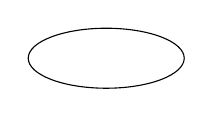
\begin{tikzpicture}

\draw (1.18in,-0.3in) ellipse [x radius=0.39in, y radius=0.15in];
\end{tikzpicture}


%%%%%%%%%%%%%%%%%%%% Figure/Image No: 17 starts here %%%%%%%%%%%%%%%%%%%%

\begin{figure}[H]
	\begin{Center}
		\includegraphics[width=4.48in,height=3.75in]{./media/image18.png}
	\end{Center}
\end{figure}


%%%%%%%%%%%%%%%%%%%% Figure/Image No: 17 Ends here %%%%%%%%%%%%%%%%%%%%

\par


\vspace{\baselineskip}
Ici, la fonction tricks est un pont entre le type String et le type TourMagie. Sachant qu’il est défini par implicit, on a plus besoin de déclarer la classe par implicit ce qui ne nous empêche pas d’utiliser les méthodes qui y ont été défini. \par


\vspace{\baselineskip}
\section*{L’utilité}
\addcontentsline{toc}{section}{L’utilité}

\vspace{\baselineskip}
En gros scala implicit permet de laisser au compilateur d’aller chercher lui-même les éléments qui lui manque au lieu que ça soit le développer qui l’indique.\par

L’utilisation de scala implicit peut être très utile lorsque vous avez besoin d’affecter la même valeur à plusieurs reprises. Cela vous permet aussi d’avoir une meilleure lisibilité du code. Les bibliothèques de scala utilisent souvent scala implicit pour définir des implémentations par défaut. \par

Il y a aussi des inconvénients avec cet outils. Malgré le fait qu’il facilite la lecture d’un code, déboguer un code devient assez compliqué. On peut très facilement tomber sur des cas d’ambiguïté avec les paramètres implicit. Lorsqu’on utilise des classes implicit on ne peut affecter le même nom pour deux méthodes appartenant à deux classes différentes car ça créée une ambiguïté. \par


\printbibliography
\end{document}
